\documentclass[1p]{elsarticle_modified}
%\bibliographystyle{elsarticle-num}

%\usepackage[colorlinks]{hyperref}
%\usepackage{abbrmath_seonhwa} %\Abb, \Ascr, \Acal ,\Abf, \Afrak
\usepackage{amsfonts}
\usepackage{amssymb}
\usepackage{amsmath}
\usepackage{amsthm}
\usepackage{scalefnt}
\usepackage{amsbsy}
\usepackage{kotex}
\usepackage{caption}
\usepackage{subfig}
\usepackage{color}
\usepackage{graphicx}
\usepackage{xcolor} %% white, black, red, green, blue, cyan, magenta, yellow
\usepackage{float}
\usepackage{setspace}
\usepackage{hyperref}

\usepackage{tikz}
\usetikzlibrary{arrows}

\usepackage{multirow}
\usepackage{array} % fixed length table
\usepackage{hhline}

%%%%%%%%%%%%%%%%%%%%%
\makeatletter
\renewcommand*\env@matrix[1][\arraystretch]{%
	\edef\arraystretch{#1}%
	\hskip -\arraycolsep
	\let\@ifnextchar\new@ifnextchar
	\array{*\c@MaxMatrixCols c}}
\makeatother %https://tex.stackexchange.com/questions/14071/how-can-i-increase-the-line-spacing-in-a-matrix
%%%%%%%%%%%%%%%

\usepackage[normalem]{ulem}

\newcommand{\msout}[1]{\ifmmode\text{\sout{\ensuremath{#1}}}\else\sout{#1}\fi}
%SOURCE: \msout is \stkout macro in https://tex.stackexchange.com/questions/20609/strikeout-in-math-mode

\newcommand{\cancel}[1]{
	\ifmmode
	{\color{red}\msout{#1}}
	\else
	{\color{red}\sout{#1}}
	\fi
}

\newcommand{\add}[1]{
	{\color{blue}\uwave{#1}}
}

\newcommand{\replace}[2]{
	\ifmmode
	{\color{red}\msout{#1}}{\color{blue}\uwave{#2}}
	\else
	{\color{red}\sout{#1}}{\color{blue}\uwave{#2}}
	\fi
}

\newcommand{\Sol}{\mathcal{S}} %segment
\newcommand{\D}{D} %diagram
\newcommand{\A}{\mathcal{A}} %arc


%%%%%%%%%%%%%%%%%%%%%%%%%%%%%5 test

\def\sl{\operatorname{\textup{SL}}(2,\Cbb)}
\def\psl{\operatorname{\textup{PSL}}(2,\Cbb)}
\def\quan{\mkern 1mu \triangleright \mkern 1mu}

\theoremstyle{definition}
\newtheorem{thm}{Theorem}[section]
\newtheorem{prop}[thm]{Proposition}
\newtheorem{lem}[thm]{Lemma}
\newtheorem{ques}[thm]{Question}
\newtheorem{cor}[thm]{Corollary}
\newtheorem{defn}[thm]{Definition}
\newtheorem{exam}[thm]{Example}
\newtheorem{rmk}[thm]{Remark}
\newtheorem{alg}[thm]{Algorithm}

\newcommand{\I}{\sqrt{-1}}
\begin{document}

%\begin{frontmatter}
%
%\title{Boundary parabolic representations of knots up to 8 crossings}
%
%%% Group authors per affiliation:
%\author{Yunhi Cho} 
%\address{Department of Mathematics, University of Seoul, Seoul, Korea}
%\ead{yhcho@uos.ac.kr}
%
%
%\author{Seonhwa Kim} %\fnref{s_kim}}
%\address{Center for Geometry and Physics, Institute for Basic Science, Pohang, 37673, Korea}
%\ead{ryeona17@ibs.re.kr}
%
%\author{Hyuk Kim}
%\address{Department of Mathematical Sciences, Seoul National University, Seoul 08826, Korea}
%\ead{hyukkim@snu.ac.kr}
%
%\author{Seokbeom Yoon}
%\address{Department of Mathematical Sciences, Seoul National University, Seoul, 08826,  Korea}
%\ead{sbyoon15@snu.ac.kr}
%
%\begin{abstract}
%We find all boundary parabolic representation of knots up to 8 crossings.
%
%\end{abstract}
%\begin{keyword}
%    \MSC[2010] 57M25 
%\end{keyword}
%
%\end{frontmatter}

%\linenumbers
%\tableofcontents
%
\newcommand\colored[1]{\textcolor{white}{\rule[-0.35ex]{0.8em}{1.4ex}}\kern-0.8em\color{red} #1}%
%\newcommand\colored[1]{\textcolor{white}{ #1}\kern-2.17ex	\textcolor{white}{ #1}\kern-1.81ex	\textcolor{white}{ #1}\kern-2.15ex\color{red}#1	}

{\Large $\underline{12n_{0602}~(K12n_{0602})}$}

\setlength{\tabcolsep}{10pt}
\renewcommand{\arraystretch}{1.6}
\vspace{1cm}\begin{tabular}{m{100pt}>{\centering\arraybackslash}m{274pt}}
\multirow{5}{120pt}{
	\centering
	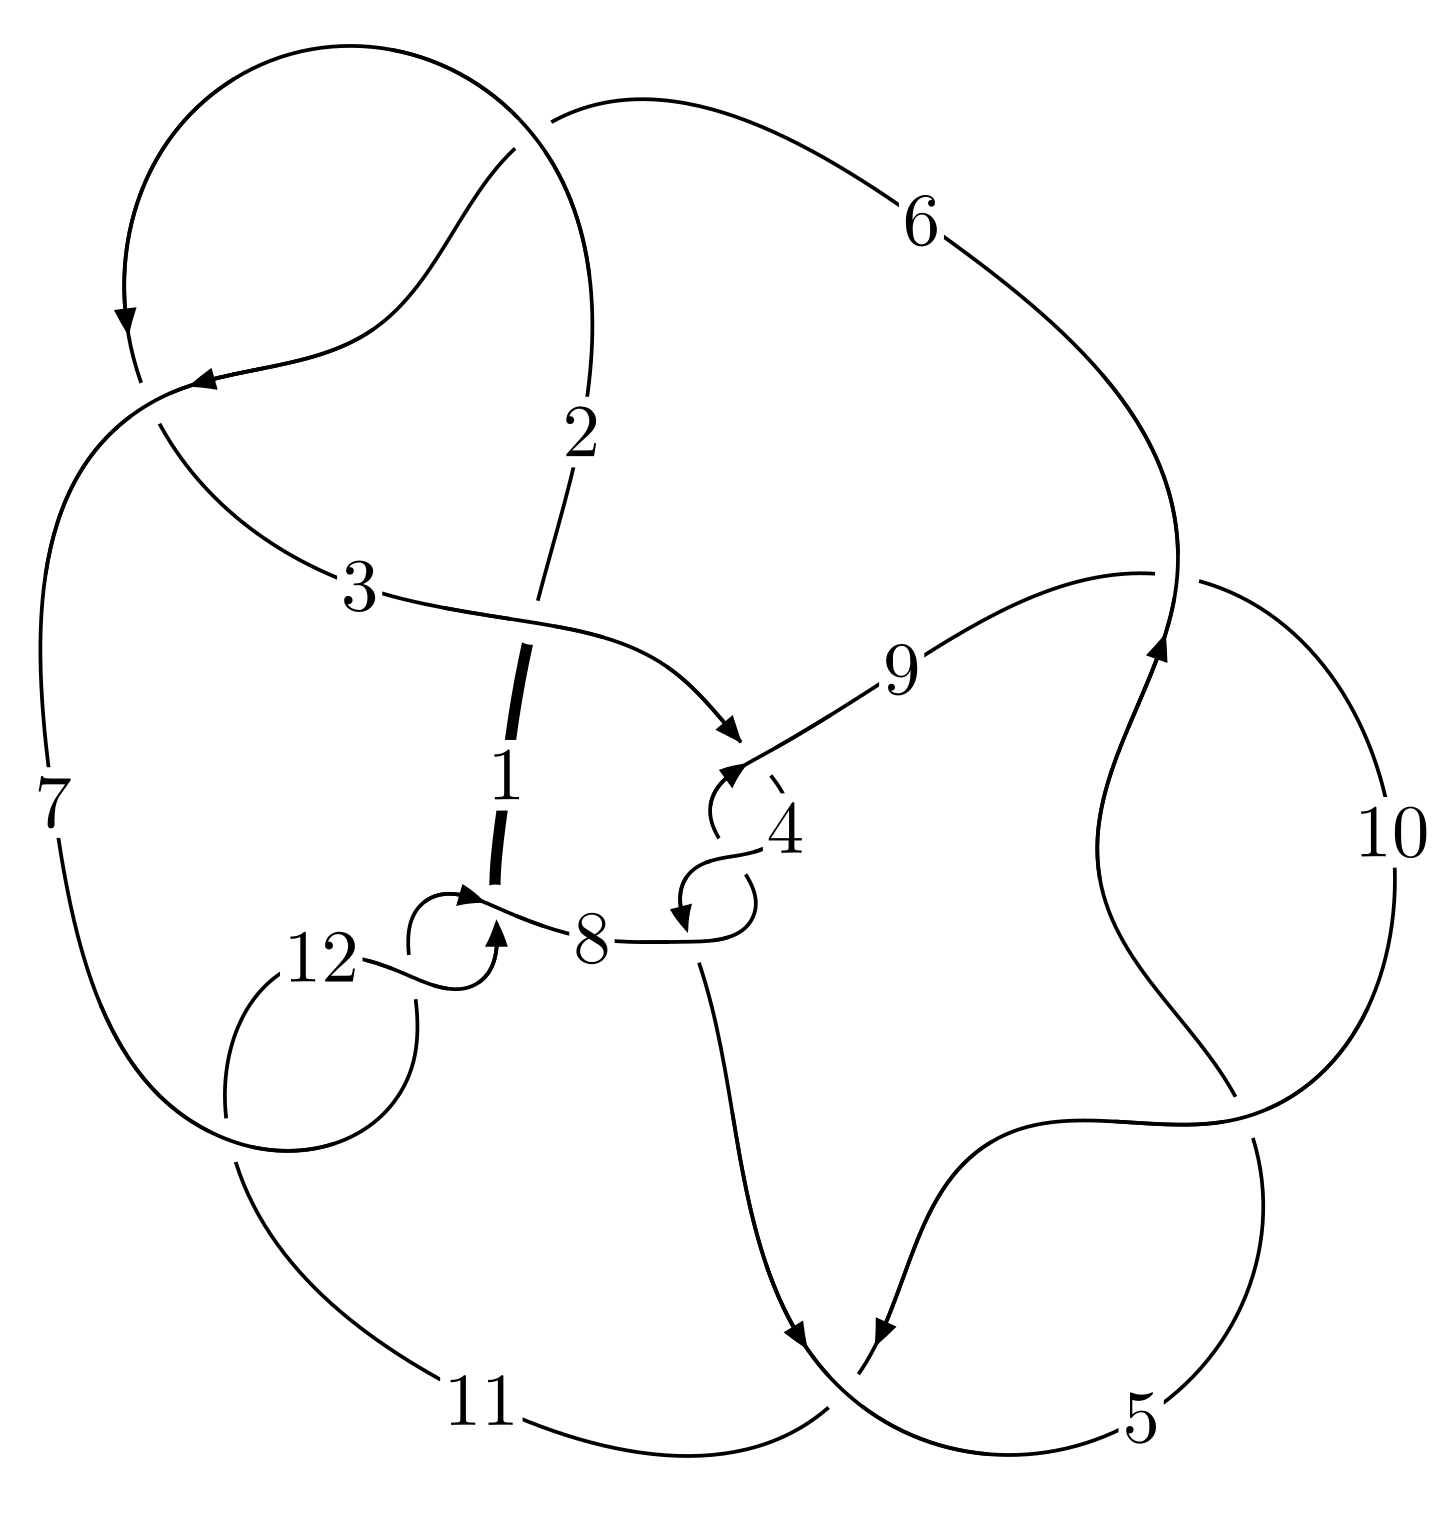
\includegraphics[width=112pt]{../../../GIT/diagram.site/Diagrams/png/2691_12n_0602.png}\\
\ \ \ A knot diagram\footnotemark}&
\allowdisplaybreaks
\textbf{Linearized knot diagam} \\
\cline{2-2}
 &
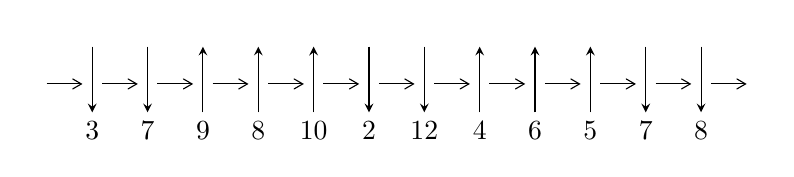
\begin{tikzpicture}[x=20pt, y=17pt]
	% nodes
	\node (C0) at (0, 0) {};
	\node (C1) at (1, 0) {};
	\node (C1U) at (1, +1) {};
	\node (C1D) at (1, -1) {3};

	\node (C2) at (2, 0) {};
	\node (C2U) at (2, +1) {};
	\node (C2D) at (2, -1) {7};

	\node (C3) at (3, 0) {};
	\node (C3U) at (3, +1) {};
	\node (C3D) at (3, -1) {9};

	\node (C4) at (4, 0) {};
	\node (C4U) at (4, +1) {};
	\node (C4D) at (4, -1) {8};

	\node (C5) at (5, 0) {};
	\node (C5U) at (5, +1) {};
	\node (C5D) at (5, -1) {10};

	\node (C6) at (6, 0) {};
	\node (C6U) at (6, +1) {};
	\node (C6D) at (6, -1) {2};

	\node (C7) at (7, 0) {};
	\node (C7U) at (7, +1) {};
	\node (C7D) at (7, -1) {12};

	\node (C8) at (8, 0) {};
	\node (C8U) at (8, +1) {};
	\node (C8D) at (8, -1) {4};

	\node (C9) at (9, 0) {};
	\node (C9U) at (9, +1) {};
	\node (C9D) at (9, -1) {6};

	\node (C10) at (10, 0) {};
	\node (C10U) at (10, +1) {};
	\node (C10D) at (10, -1) {5};

	\node (C11) at (11, 0) {};
	\node (C11U) at (11, +1) {};
	\node (C11D) at (11, -1) {7};

	\node (C12) at (12, 0) {};
	\node (C12U) at (12, +1) {};
	\node (C12D) at (12, -1) {8};
	\node (C13) at (13, 0) {};

	% arrows
	\draw[->,>={angle 60}]
	(C0) edge (C1) (C1) edge (C2) (C2) edge (C3) (C3) edge (C4) (C4) edge (C5) (C5) edge (C6) (C6) edge (C7) (C7) edge (C8) (C8) edge (C9) (C9) edge (C10) (C10) edge (C11) (C11) edge (C12) (C12) edge (C13) ;	\draw[->,>=stealth]
	(C1U) edge (C1D) (C2U) edge (C2D) (C3D) edge (C3U) (C4D) edge (C4U) (C5D) edge (C5U) (C6U) edge (C6D) (C7U) edge (C7D) (C8D) edge (C8U) (C9D) edge (C9U) (C10D) edge (C10U) (C11U) edge (C11D) (C12U) edge (C12D) ;
	\end{tikzpicture} \\
\hhline{~~} \\& 
\textbf{Solving Sequence} \\ \cline{2-2} 
 &
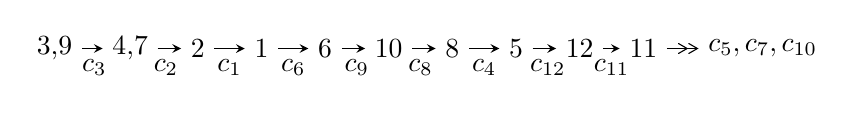
\begin{tikzpicture}[x=23pt, y=7pt]
	% node
	\node (A0) at (-1/8, 0) {3,9};
	\node (A1) at (17/16, 0) {4,7};
	\node (A2) at (17/8, 0) {2};
	\node (A3) at (25/8, 0) {1};
	\node (A4) at (33/8, 0) {6};
	\node (A5) at (41/8, 0) {10};
	\node (A6) at (49/8, 0) {8};
	\node (A7) at (57/8, 0) {5};
	\node (A8) at (65/8, 0) {12};
	\node (A9) at (73/8, 0) {11};
	\node (C1) at (1/2, -1) {$c_{3}$};
	\node (C2) at (13/8, -1) {$c_{2}$};
	\node (C3) at (21/8, -1) {$c_{1}$};
	\node (C4) at (29/8, -1) {$c_{6}$};
	\node (C5) at (37/8, -1) {$c_{9}$};
	\node (C6) at (45/8, -1) {$c_{8}$};
	\node (C7) at (53/8, -1) {$c_{4}$};
	\node (C8) at (61/8, -1) {$c_{12}$};
	\node (C9) at (69/8, -1) {$c_{11}$};
	\node (A10) at (11, 0) {$c_{5},c_{7},c_{10}$};

	% edge
	\draw[->,>=stealth]	
	(A0) edge (A1) (A1) edge (A2) (A2) edge (A3) (A3) edge (A4) (A4) edge (A5) (A5) edge (A6) (A6) edge (A7) (A7) edge (A8) (A8) edge (A9) ;
	\draw[->>,>={angle 60}]	
	(A9) edge (A10);
\end{tikzpicture} \\ 

\end{tabular} \\

\footnotetext{
The image of knot diagram is generated by the software ``\textbf{Draw programme}" developed by Andrew Bartholomew(\url{http://www.layer8.co.uk/maths/draw/index.htm\#Running-draw}), where we modified some parts for our purpose(\url{https://github.com/CATsTAILs/LinksPainter}).
}\phantom \\ \newline 
\centering \textbf{Ideals for irreducible components\footnotemark of $X_{\text{par}}$} 
 
\begin{align*}
I^u_{1}&=\langle 
- u^9-3 u^8-7 u^7-10 u^6-9 u^5+2 u^4+5 u^3+11 u^2+8 b-6 u-2,\\
\phantom{I^u_{1}}&\phantom{= \langle  }u^8+5 u^6- u^5+6 u^4-2 u^3+u^2+4 a+2 u-2,\;u^{10}+6 u^8-3 u^7+11 u^6-13 u^5+9 u^4-12 u^3+7 u^2+2\rangle \\
I^u_{2}&=\langle 
-937 u^{13}-2472 u^{12}+\cdots+1987 b-6836,\;12531 u^{13}+27338 u^{12}+\cdots+19870 a+85927,\\
\phantom{I^u_{2}}&\phantom{= \langle  }u^{14}+3 u^{13}+\cdots+22 u+5\rangle \\
I^u_{3}&=\langle 
- u^4 a- u^2 a- u^3- a u+b+a- u-1,\\
\phantom{I^u_{3}}&\phantom{= \langle  }-2 u^5 a-2 u^4 a+u^5-6 u^3 a+u^4-6 u^2 a+2 u^3+2 a^2-6 a u+3 u^2-6 a+u+3,\\
\phantom{I^u_{3}}&\phantom{= \langle  }u^6+3 u^4+u^3+2 u^2+2 u-1\rangle \\
I^u_{4}&=\langle 
2 u^9 a+10 u^9+\cdots+7 a+1,\;-2 u^9+3 u^8+\cdots+a^2-4,\;u^{10}- u^9+4 u^8-4 u^7+6 u^6-6 u^5+3 u^4-3 u^3+1\rangle \\
I^u_{5}&=\langle 
b-1,\;6 a- u-3,\;u^2+3\rangle \\
I^u_{6}&=\langle 
b- u,\;2 a+u+1,\;u^2+1\rangle \\
\\
I^v_{1}&=\langle 
a,\;b-1,\;v+1\rangle \\
\end{align*}
\raggedright * 7 irreducible components of $\dim_{\mathbb{C}}=0$, with total 61 representations.\\
\footnotetext{All coefficients of polynomials are rational numbers. But the coefficients are sometimes approximated in decimal forms when there is not enough margin.}
\newpage
\renewcommand{\arraystretch}{1}
\centering \section*{I. $I^u_{1}= \langle - u^9-3 u^8+\cdots+8 b-2,\;u^8+5 u^6- u^5+6 u^4-2 u^3+u^2+4 a+2 u-2,\;u^{10}+6 u^8+\cdots+7 u^2+2 \rangle$}
\flushleft \textbf{(i) Arc colorings}\\
\begin{tabular}{m{7pt} m{180pt} m{7pt} m{180pt} }
\flushright $a_{3}=$&$\begin{pmatrix}1\\0\end{pmatrix}$ \\
\flushright $a_{9}=$&$\begin{pmatrix}0\\u\end{pmatrix}$ \\
\flushright $a_{4}=$&$\begin{pmatrix}1\\- u^2\end{pmatrix}$ \\
\flushright $a_{7}=$&$\begin{pmatrix}-\frac{1}{4} u^8-\frac{5}{4} u^6+\cdots-\frac{1}{2} u+\frac{1}{2}\\\frac{1}{8} u^9+\frac{3}{8} u^8+\cdots+\frac{3}{4} u+\frac{1}{4}\end{pmatrix}$ \\
\flushright $a_{2}=$&$\begin{pmatrix}-\frac{1}{4} u^8-\frac{5}{4} u^6+\cdots-\frac{1}{2} u+\frac{1}{2}\\-\frac{3}{8} u^9+\frac{3}{8} u^8+\cdots-\frac{5}{4} u+\frac{1}{4}\end{pmatrix}$ \\
\flushright $a_{1}=$&$\begin{pmatrix}-\frac{3}{8} u^9+\frac{1}{8} u^8+\cdots-\frac{7}{4} u+\frac{3}{4}\\-\frac{3}{8} u^9+\frac{3}{8} u^8+\cdots-\frac{5}{4} u+\frac{1}{4}\end{pmatrix}$ \\
\flushright $a_{6}=$&$\begin{pmatrix}1\\\frac{1}{2} u^9+\frac{1}{2} u^8+\cdots+u+1\end{pmatrix}$ \\
\flushright $a_{10}=$&$\begin{pmatrix}u\\\frac{1}{2} u^9-\frac{1}{2} u^8+\cdots+2 u-1\end{pmatrix}$ \\
\flushright $a_{8}=$&$\begin{pmatrix}- u\\u^3+u\end{pmatrix}$ \\
\flushright $a_{5}=$&$\begin{pmatrix}u^2+1\\- u^4-2 u^2\end{pmatrix}$ \\
\flushright $a_{12}=$&$\begin{pmatrix}\frac{1}{4} u^8+\frac{5}{4} u^6+\cdots-\frac{3}{2} u+\frac{1}{2}\\-\frac{1}{8} u^9+\frac{1}{8} u^8+\cdots-\frac{3}{4} u+\frac{3}{4}\end{pmatrix}$ \\
\flushright $a_{11}=$&$\begin{pmatrix}- u^3-2 u\\-\frac{1}{2} u^9+\frac{1}{2} u^8+\cdots-2 u+1\end{pmatrix}$\\&\end{tabular}
\flushleft \textbf{(ii) Obstruction class $= -1$}\\~\\
\flushleft \textbf{(iii) Cusp Shapes $= \frac{3}{2} u^9-\frac{1}{2} u^8+\frac{17}{2} u^7-8 u^6+\frac{25}{2} u^5-25 u^4+\frac{17}{2} u^3-\frac{27}{2} u^2+13 u+1$}\\~\\
\newpage\renewcommand{\arraystretch}{1}
\flushleft \textbf{(iv) u-Polynomials at the component}\newline \\
\begin{tabular}{m{50pt}|m{274pt}}
Crossings & \hspace{64pt}u-Polynomials at each crossing \\
\hline $$\begin{aligned}c_{1}\end{aligned}$$&$\begin{aligned}
&u^{10}+u^9+2 u^8-3 u^7+12 u^6+24 u^5+46 u^4+37 u^3+7 u^2-3 u+4
\end{aligned}$\\
\hline $$\begin{aligned}c_{2},c_{6},c_{7}\\c_{11},c_{12}\end{aligned}$$&$\begin{aligned}
&u^{10}-3 u^9+4 u^8- u^7-4 u^6+6 u^5-3 u^3+u^2+u+2
\end{aligned}$\\
\hline $$\begin{aligned}c_{3},c_{4},c_{5}\\c_{8},c_{9},c_{10}\end{aligned}$$&$\begin{aligned}
&u^{10}+6 u^8+3 u^7+11 u^6+13 u^5+9 u^4+12 u^3+7 u^2+2
\end{aligned}$\\
\hline
\end{tabular}\\~\\
\newpage\renewcommand{\arraystretch}{1}
\flushleft \textbf{(v) Riley Polynomials at the component}\newline \\
\begin{tabular}{m{50pt}|m{274pt}}
Crossings & \hspace{64pt}Riley Polynomials at each crossing \\
\hline $$\begin{aligned}c_{1}\end{aligned}$$&$\begin{aligned}
&y^{10}+3 y^9+\cdots+47 y+16
\end{aligned}$\\
\hline $$\begin{aligned}c_{2},c_{6},c_{7}\\c_{11},c_{12}\end{aligned}$$&$\begin{aligned}
&y^{10}- y^9+2 y^8+3 y^7+12 y^6-24 y^5+46 y^4-37 y^3+7 y^2+3 y+4
\end{aligned}$\\
\hline $$\begin{aligned}c_{3},c_{4},c_{5}\\c_{8},c_{9},c_{10}\end{aligned}$$&$\begin{aligned}
&y^{10}+12 y^9+\cdots+28 y+4
\end{aligned}$\\
\hline
\end{tabular}\\~\\
\newpage\flushleft \textbf{(vi) Complex Volumes and Cusp Shapes}
$$\begin{array}{c|c|c}  
\text{Solutions to }I^u_{1}& \I (\text{vol} + \sqrt{-1}CS) & \text{Cusp shape}\\
 \hline 
\begin{aligned}
u &= \phantom{-}0.849669 + 0.278925 I \\
a &= \phantom{-}0.126908 - 1.402190 I \\
b &= -0.935978 + 0.707374 I\end{aligned}
 & \phantom{-}2.59736 + 5.48528 I & \phantom{-}0.63906 - 6.67204 I \\ \hline\begin{aligned}
u &= \phantom{-}0.849669 - 0.278925 I \\
a &= \phantom{-}0.126908 + 1.402190 I \\
b &= -0.935978 - 0.707374 I\end{aligned}
 & \phantom{-}2.59736 - 5.48528 I & \phantom{-}0.63906 + 6.67204 I \\ \hline\begin{aligned}
u &= -0.179655 + 1.191160 I \\
a &= \phantom{-}0.250838 - 0.636140 I \\
b &= -0.46356 + 1.36046 I\end{aligned}
 & -2.21767 - 1.59735 I & -7.51312 + 4.64580 I \\ \hline\begin{aligned}
u &= -0.179655 - 1.191160 I \\
a &= \phantom{-}0.250838 + 0.636140 I \\
b &= -0.46356 - 1.36046 I\end{aligned}
 & -2.21767 + 1.59735 I & -7.51312 - 4.64580 I \\ \hline\begin{aligned}
u &= -0.44148 + 1.44610 I \\
a &= -0.552527 + 1.275850 I \\
b &= -1.28583 - 0.66001 I\end{aligned}
 & -8.2686 - 15.1646 I & -7.51854 + 8.25672 I \\ \hline\begin{aligned}
u &= -0.44148 - 1.44610 I \\
a &= -0.552527 - 1.275850 I \\
b &= -1.28583 + 0.66001 I\end{aligned}
 & -8.2686 + 15.1646 I & -7.51854 - 8.25672 I \\ \hline\begin{aligned}
u &= -0.171957 + 0.454648 I \\
a &= \phantom{-}0.655512 - 0.286314 I \\
b &= \phantom{-}0.281118 + 0.559566 I\end{aligned}
 & \phantom{-}0.087563 - 1.088810 I & \phantom{-}1.48967 + 6.22992 I \\ \hline\begin{aligned}
u &= -0.171957 - 0.454648 I \\
a &= \phantom{-}0.655512 + 0.286314 I \\
b &= \phantom{-}0.281118 - 0.559566 I\end{aligned}
 & \phantom{-}0.087563 + 1.088810 I & \phantom{-}1.48967 - 6.22992 I \\ \hline\begin{aligned}
u &= -0.05658 + 1.78531 I \\
a &= \phantom{-}0.519269 + 0.055233 I \\
b &= \phantom{-}0.904241 - 0.202548 I\end{aligned}
 & -16.0502 + 0.8822 I & -5.09706 - 8.51458 I \\ \hline\begin{aligned}
u &= -0.05658 - 1.78531 I \\
a &= \phantom{-}0.519269 - 0.055233 I \\
b &= \phantom{-}0.904241 + 0.202548 I\end{aligned}
 & -16.0502 - 0.8822 I & -5.09706 + 8.51458 I\\
 \hline 
 \end{array}$$\newpage\newpage\renewcommand{\arraystretch}{1}
\centering \section*{II. $I^u_{2}= \langle -937 u^{13}-2472 u^{12}+\cdots+1987 b-6836,\;12531 u^{13}+27338 u^{12}+\cdots+19870 a+85927,\;u^{14}+3 u^{13}+\cdots+22 u+5 \rangle$}
\flushleft \textbf{(i) Arc colorings}\\
\begin{tabular}{m{7pt} m{180pt} m{7pt} m{180pt} }
\flushright $a_{3}=$&$\begin{pmatrix}1\\0\end{pmatrix}$ \\
\flushright $a_{9}=$&$\begin{pmatrix}0\\u\end{pmatrix}$ \\
\flushright $a_{4}=$&$\begin{pmatrix}1\\- u^2\end{pmatrix}$ \\
\flushright $a_{7}=$&$\begin{pmatrix}-0.630649 u^{13}-1.37584 u^{12}+\cdots-15.3917 u-4.32446\\0.471565 u^{13}+1.24409 u^{12}+\cdots+9.17765 u+3.44036\end{pmatrix}$ \\
\flushright $a_{2}=$&$\begin{pmatrix}0.253296 u^{13}+0.379668 u^{12}+\cdots+0.855511 u+0.00558631\\-0.425264 u^{13}-0.827378 u^{12}+\cdots-8.90941 u-2.81228\end{pmatrix}$ \\
\flushright $a_{1}=$&$\begin{pmatrix}-0.171968 u^{13}-0.447710 u^{12}+\cdots-8.05390 u-2.80669\\-0.425264 u^{13}-0.827378 u^{12}+\cdots-8.90941 u-2.81228\end{pmatrix}$ \\
\flushright $a_{6}=$&$\begin{pmatrix}-0.693105 u^{13}-1.63795 u^{12}+\cdots-20.3068 u-6.28908\\0.351787 u^{13}+1.16608 u^{12}+\cdots+6.24459 u+3.20684\end{pmatrix}$ \\
\flushright $a_{10}=$&$\begin{pmatrix}-0.241369 u^{13}-0.372320 u^{12}+\cdots-0.359235 u+0.934474\\0.330649 u^{13}+0.975843 u^{12}+\cdots+16.4917 u+5.22446\end{pmatrix}$ \\
\flushright $a_{8}=$&$\begin{pmatrix}- u\\u^3+u\end{pmatrix}$ \\
\flushright $a_{5}=$&$\begin{pmatrix}u^2+1\\- u^4-2 u^2\end{pmatrix}$ \\
\flushright $a_{12}=$&$\begin{pmatrix}-0.342577 u^{13}-0.983191 u^{12}+\cdots-14.9880 u-5.16452\\-0.112733 u^{13}-0.0145949 u^{12}+\cdots-3.34877 u-0.572723\end{pmatrix}$ \\
\flushright $a_{11}=$&$\begin{pmatrix}-0.0892803 u^{13}-0.603523 u^{12}+\cdots-14.1325 u-6.15893\\-0.537997 u^{13}-0.841973 u^{12}+\cdots-12.2582 u-3.38500\end{pmatrix}$\\&\end{tabular}
\flushleft \textbf{(ii) Obstruction class $= -1$}\\~\\
\flushleft \textbf{(iii) Cusp Shapes $= \frac{2058}{1987} u^{13}+\frac{6600}{1987} u^{12}+\cdots+\frac{37538}{1987} u+\frac{12194}{1987}$}\\~\\
\newpage\renewcommand{\arraystretch}{1}
\flushleft \textbf{(iv) u-Polynomials at the component}\newline \\
\begin{tabular}{m{50pt}|m{274pt}}
Crossings & \hspace{64pt}u-Polynomials at each crossing \\
\hline $$\begin{aligned}c_{1}\end{aligned}$$&$\begin{aligned}
&(u^7+3 u^6+7 u^5+8 u^4+9 u^3+6 u^2+5 u+1)^2
\end{aligned}$\\
\hline $$\begin{aligned}c_{2},c_{6},c_{7}\\c_{11},c_{12}\end{aligned}$$&$\begin{aligned}
&(u^7+u^6- u^5-2 u^4+u^3+2 u^2+u-1)^2
\end{aligned}$\\
\hline $$\begin{aligned}c_{3},c_{4},c_{5}\\c_{8},c_{9},c_{10}\end{aligned}$$&$\begin{aligned}
&u^{14}-3 u^{13}+\cdots-22 u+5
\end{aligned}$\\
\hline
\end{tabular}\\~\\
\newpage\renewcommand{\arraystretch}{1}
\flushleft \textbf{(v) Riley Polynomials at the component}\newline \\
\begin{tabular}{m{50pt}|m{274pt}}
Crossings & \hspace{64pt}Riley Polynomials at each crossing \\
\hline $$\begin{aligned}c_{1}\end{aligned}$$&$\begin{aligned}
&(y^7+5 y^6+19 y^5+36 y^4+49 y^3+38 y^2+13 y-1)^2
\end{aligned}$\\
\hline $$\begin{aligned}c_{2},c_{6},c_{7}\\c_{11},c_{12}\end{aligned}$$&$\begin{aligned}
&(y^7-3 y^6+7 y^5-8 y^4+9 y^3-6 y^2+5 y-1)^2
\end{aligned}$\\
\hline $$\begin{aligned}c_{3},c_{4},c_{5}\\c_{8},c_{9},c_{10}\end{aligned}$$&$\begin{aligned}
&y^{14}+11 y^{13}+\cdots-4 y+25
\end{aligned}$\\
\hline
\end{tabular}\\~\\
\newpage\flushleft \textbf{(vi) Complex Volumes and Cusp Shapes}
$$\begin{array}{c|c|c}  
\text{Solutions to }I^u_{2}& \I (\text{vol} + \sqrt{-1}CS) & \text{Cusp shape}\\
 \hline 
\begin{aligned}
u &= \phantom{-}0.370785 + 0.946704 I \\
a &= -0.209881 - 0.303567 I \\
b &= \phantom{-}0.597306 + 0.773845 I\end{aligned}
 & \phantom{-}0.562491 - 0.955395 I & \phantom{-}0.68929 + 2.37083 I \\ \hline\begin{aligned}
u &= \phantom{-}0.370785 - 0.946704 I \\
a &= -0.209881 + 0.303567 I \\
b &= \phantom{-}0.597306 - 0.773845 I\end{aligned}
 & \phantom{-}0.562491 + 0.955395 I & \phantom{-}0.68929 - 2.37083 I \\ \hline\begin{aligned}
u &= -1.022710 + 0.247588 I \\
a &= -0.520411 - 1.220230 I \\
b &= \phantom{-}1.139460 + 0.630170 I\end{aligned}
 & -2.92618 - 9.93065 I & -4.46028 + 7.33664 I \\ \hline\begin{aligned}
u &= -1.022710 - 0.247588 I \\
a &= -0.520411 + 1.220230 I \\
b &= \phantom{-}1.139460 - 0.630170 I\end{aligned}
 & -2.92618 + 9.93065 I & -4.46028 - 7.33664 I \\ \hline\begin{aligned}
u &= \phantom{-}0.306472 + 1.132160 I \\
a &= -0.482637 - 0.675154 I \\
b &= -0.502855\phantom{ +0.000000I}\end{aligned}
 & -4.24127\phantom{ +0.000000I} & -5.93921 + 0. I\phantom{ +0.000000I} \\ \hline\begin{aligned}
u &= \phantom{-}0.306472 - 1.132160 I \\
a &= -0.482637 + 0.675154 I \\
b &= -0.502855\phantom{ +0.000000I}\end{aligned}
 & -4.24127\phantom{ +0.000000I} & -5.93921 + 0. I\phantom{ +0.000000I} \\ \hline\begin{aligned}
u &= -0.736932 + 1.071510 I \\
a &= \phantom{-}0.318588 - 0.053278 I \\
b &= -0.985336 + 0.506466 I\end{aligned}
 & -5.38528 + 3.93070 I & -6.25941 - 4.87230 I \\ \hline\begin{aligned}
u &= -0.736932 - 1.071510 I \\
a &= \phantom{-}0.318588 + 0.053278 I \\
b &= -0.985336 - 0.506466 I\end{aligned}
 & -5.38528 - 3.93070 I & -6.25941 + 4.87230 I \\ \hline\begin{aligned}
u &= -0.538570 + 0.272073 I \\
a &= \phantom{-}0.71818 - 1.43908 I \\
b &= \phantom{-}0.597306 + 0.773845 I\end{aligned}
 & \phantom{-}0.562491 - 0.955395 I & \phantom{-}0.68929 + 2.37083 I \\ \hline\begin{aligned}
u &= -0.538570 - 0.272073 I \\
a &= \phantom{-}0.71818 + 1.43908 I \\
b &= \phantom{-}0.597306 - 0.773845 I\end{aligned}
 & \phantom{-}0.562491 + 0.955395 I & \phantom{-}0.68929 - 2.37083 I\\
 \hline 
 \end{array}$$\newpage$$\begin{array}{c|c|c}  
\text{Solutions to }I^u_{2}& \I (\text{vol} + \sqrt{-1}CS) & \text{Cusp shape}\\
 \hline 
\begin{aligned}
u &= \phantom{-}0.36817 + 1.45006 I \\
a &= \phantom{-}0.797752 + 1.077130 I \\
b &= \phantom{-}1.139460 - 0.630170 I\end{aligned}
 & -2.92618 + 9.93065 I & -4.46028 - 7.33664 I \\ \hline\begin{aligned}
u &= \phantom{-}0.36817 - 1.45006 I \\
a &= \phantom{-}0.797752 - 1.077130 I \\
b &= \phantom{-}1.139460 + 0.630170 I\end{aligned}
 & -2.92618 - 9.93065 I & -4.46028 + 7.33664 I \\ \hline\begin{aligned}
u &= -0.24721 + 1.49766 I \\
a &= -0.921588 + 0.632363 I \\
b &= -0.985336 - 0.506466 I\end{aligned}
 & -5.38528 - 3.93070 I & -6.25941 + 4.87230 I \\ \hline\begin{aligned}
u &= -0.24721 - 1.49766 I \\
a &= -0.921588 - 0.632363 I \\
b &= -0.985336 + 0.506466 I\end{aligned}
 & -5.38528 + 3.93070 I & -6.25941 - 4.87230 I\\
 \hline 
 \end{array}$$\newpage\newpage\renewcommand{\arraystretch}{1}
\centering \section*{III. $I^u_{3}= \langle - u^4 a- u^2 a- u^3- a u+b+a- u-1,\;-2 u^5 a+u^5+\cdots-6 a+3,\;u^6+3 u^4+u^3+2 u^2+2 u-1 \rangle$}
\flushleft \textbf{(i) Arc colorings}\\
\begin{tabular}{m{7pt} m{180pt} m{7pt} m{180pt} }
\flushright $a_{3}=$&$\begin{pmatrix}1\\0\end{pmatrix}$ \\
\flushright $a_{9}=$&$\begin{pmatrix}0\\u\end{pmatrix}$ \\
\flushright $a_{4}=$&$\begin{pmatrix}1\\- u^2\end{pmatrix}$ \\
\flushright $a_{7}=$&$\begin{pmatrix}a\\u^4 a+u^2 a+u^3+a u- a+u+1\end{pmatrix}$ \\
\flushright $a_{2}=$&$\begin{pmatrix}a\\u^5 a+2 u^3 a+u^2 a- u^3- u-1\end{pmatrix}$ \\
\flushright $a_{1}=$&$\begin{pmatrix}u^5 a+2 u^3 a+u^2 a- u^3+a- u-1\\u^5 a+2 u^3 a+u^2 a- u^3- u-1\end{pmatrix}$ \\
\flushright $a_{6}=$&$\begin{pmatrix}1\\u^5+u^4+2 u^3+2 u^2+u-1\end{pmatrix}$ \\
\flushright $a_{10}=$&$\begin{pmatrix}u\\u^5- u^4+u^3- u^2-2 u+1\end{pmatrix}$ \\
\flushright $a_{8}=$&$\begin{pmatrix}- u\\u^3+u\end{pmatrix}$ \\
\flushright $a_{5}=$&$\begin{pmatrix}u^2+1\\- u^4-2 u^2\end{pmatrix}$ \\
\flushright $a_{12}=$&$\begin{pmatrix}u^3 a- u^3+a u+a-2 u-1\\-1\end{pmatrix}$ \\
\flushright $a_{11}=$&$\begin{pmatrix}- u^3-2 u\\u^4+u^3+u^2+2 u-1\end{pmatrix}$\\&\end{tabular}
\flushleft \textbf{(ii) Obstruction class $= -1$}\\~\\
\flushleft \textbf{(iii) Cusp Shapes $= 4 u^5+4 u^4+8 u^3+12 u^2+4 u+2$}\\~\\
\newpage\renewcommand{\arraystretch}{1}
\flushleft \textbf{(iv) u-Polynomials at the component}\newline \\
\begin{tabular}{m{50pt}|m{274pt}}
Crossings & \hspace{64pt}u-Polynomials at each crossing \\
\hline $$\begin{aligned}c_{1}\end{aligned}$$&$\begin{aligned}
&u^{12}+7 u^{11}+\cdots+438 u+169
\end{aligned}$\\
\hline $$\begin{aligned}c_{2},c_{6},c_{7}\\c_{11},c_{12}\end{aligned}$$&$\begin{aligned}
&u^{12}-3 u^{11}+\cdots+42 u-13
\end{aligned}$\\
\hline $$\begin{aligned}c_{3},c_{4},c_{5}\\c_{8},c_{9},c_{10}\end{aligned}$$&$\begin{aligned}
&(u^6+3 u^4- u^3+2 u^2-2 u-1)^2
\end{aligned}$\\
\hline
\end{tabular}\\~\\
\newpage\renewcommand{\arraystretch}{1}
\flushleft \textbf{(v) Riley Polynomials at the component}\newline \\
\begin{tabular}{m{50pt}|m{274pt}}
Crossings & \hspace{64pt}Riley Polynomials at each crossing \\
\hline $$\begin{aligned}c_{1}\end{aligned}$$&$\begin{aligned}
&y^{12}-3 y^{11}+\cdots-59686 y+28561
\end{aligned}$\\
\hline $$\begin{aligned}c_{2},c_{6},c_{7}\\c_{11},c_{12}\end{aligned}$$&$\begin{aligned}
&y^{12}-7 y^{11}+\cdots-438 y+169
\end{aligned}$\\
\hline $$\begin{aligned}c_{3},c_{4},c_{5}\\c_{8},c_{9},c_{10}\end{aligned}$$&$\begin{aligned}
&(y^6+6 y^5+13 y^4+9 y^3-6 y^2-8 y+1)^2
\end{aligned}$\\
\hline
\end{tabular}\\~\\
\newpage\flushleft \textbf{(vi) Complex Volumes and Cusp Shapes}
$$\begin{array}{c|c|c}  
\text{Solutions to }I^u_{3}& \I (\text{vol} + \sqrt{-1}CS) & \text{Cusp shape}\\
 \hline 
\begin{aligned}
u &= -0.841864\phantom{ +0.000000I} \\
a &= \phantom{-}0.445035 + 1.177780 I \\
b &= -0.719261 - 0.742974 I\end{aligned}
 & \phantom{-}3.23778\phantom{ +0.000000I} & \phantom{-}2.68180\phantom{ +0.000000I} \\ \hline\begin{aligned}
u &= -0.841864\phantom{ +0.000000I} \\
a &= \phantom{-}0.445035 - 1.177780 I \\
b &= -0.719261 + 0.742974 I\end{aligned}
 & \phantom{-}3.23778\phantom{ +0.000000I} & \phantom{-}2.68180\phantom{ +0.000000I} \\ \hline\begin{aligned}
u &= -0.126468 + 1.352400 I \\
a &= -0.034921 + 1.148040 I \\
b &= -1.026470 - 0.870245 I\end{aligned}
 & -11.65360 - 3.39374 I & -10.36018 + 3.51762 I \\ \hline\begin{aligned}
u &= -0.126468 + 1.352400 I \\
a &= \phantom{-}0.383840 + 0.027542 I \\
b &= \phantom{-}1.59190 - 0.18598 I\end{aligned}
 & -11.65360 - 3.39374 I & -10.36018 + 3.51762 I \\ \hline\begin{aligned}
u &= -0.126468 - 1.352400 I \\
a &= -0.034921 - 1.148040 I \\
b &= -1.026470 + 0.870245 I\end{aligned}
 & -11.65360 + 3.39374 I & -10.36018 - 3.51762 I \\ \hline\begin{aligned}
u &= -0.126468 - 1.352400 I \\
a &= \phantom{-}0.383840 - 0.027542 I \\
b &= \phantom{-}1.59190 + 0.18598 I\end{aligned}
 & -11.65360 + 3.39374 I & -10.36018 - 3.51762 I \\ \hline\begin{aligned}
u &= \phantom{-}0.376468 + 1.319680 I \\
a &= -0.443330 - 1.186910 I \\
b &= -1.27617 + 0.73937 I\end{aligned}
 & -5.05799 + 8.77346 I & -5.56216 - 5.90094 I \\ \hline\begin{aligned}
u &= \phantom{-}0.376468 + 1.319680 I \\
a &= \phantom{-}0.392175 + 0.613857 I \\
b &= -0.260915 - 1.156860 I\end{aligned}
 & -5.05799 + 8.77346 I & -5.56216 - 5.90094 I \\ \hline\begin{aligned}
u &= \phantom{-}0.376468 - 1.319680 I \\
a &= -0.443330 + 1.186910 I \\
b &= -1.27617 - 0.73937 I\end{aligned}
 & -5.05799 - 8.77346 I & -5.56216 + 5.90094 I \\ \hline\begin{aligned}
u &= \phantom{-}0.376468 - 1.319680 I \\
a &= \phantom{-}0.392175 - 0.613857 I \\
b &= -0.260915 + 1.156860 I\end{aligned}
 & -5.05799 - 8.77346 I & -5.56216 + 5.90094 I\\
 \hline 
 \end{array}$$\newpage$$\begin{array}{c|c|c}  
\text{Solutions to }I^u_{3}& \I (\text{vol} + \sqrt{-1}CS) & \text{Cusp shape}\\
 \hline 
\begin{aligned}
u &= \phantom{-}0.341865\phantom{ +0.000000I} \\
a &= \phantom{-}0.468459\phantom{ +0.000000I} \\
b &= \phantom{-}1.13466\phantom{ +0.000000I}\end{aligned}
 & -2.71328\phantom{ +0.000000I} & \phantom{-}5.16290\phantom{ +0.000000I} \\ \hline\begin{aligned}
u &= \phantom{-}0.341865\phantom{ +0.000000I} \\
a &= \phantom{-}4.04594\phantom{ +0.000000I} \\
b &= -0.752839\phantom{ +0.000000I}\end{aligned}
 & -2.71328\phantom{ +0.000000I} & \phantom{-}5.16290\phantom{ +0.000000I}\\
 \hline 
 \end{array}$$\newpage\newpage\renewcommand{\arraystretch}{1}
\centering \section*{IV. $I^u_{4}= \langle 2 u^9 a+10 u^9+\cdots+7 a+1,\;-2 u^9+3 u^8+\cdots+a^2-4,\;u^{10}- u^9+\cdots-3 u^3+1 \rangle$}
\flushleft \textbf{(i) Arc colorings}\\
\begin{tabular}{m{7pt} m{180pt} m{7pt} m{180pt} }
\flushright $a_{3}=$&$\begin{pmatrix}1\\0\end{pmatrix}$ \\
\flushright $a_{9}=$&$\begin{pmatrix}0\\u\end{pmatrix}$ \\
\flushright $a_{4}=$&$\begin{pmatrix}1\\- u^2\end{pmatrix}$ \\
\flushright $a_{7}=$&$\begin{pmatrix}a\\-0.117647 a u^{9}-0.588235 u^{9}+\cdots-0.411765 a-0.0588235\end{pmatrix}$ \\
\flushright $a_{2}=$&$\begin{pmatrix}-0.588235 a u^{9}+0.0588235 u^{9}+\cdots-0.0588235 a+2.70588\\0.176471 a u^{9}-0.117647 u^{9}+\cdots+0.117647 a-1.41176\end{pmatrix}$ \\
\flushright $a_{1}=$&$\begin{pmatrix}-0.411765 a u^{9}-0.0588235 u^{9}+\cdots+0.0588235 a+1.29412\\0.176471 a u^{9}-0.117647 u^{9}+\cdots+0.117647 a-1.41176\end{pmatrix}$ \\
\flushright $a_{6}=$&$\begin{pmatrix}- u^9-4 u^7-5 u^5+3 u\\u^9+3 u^7+3 u^5- u\end{pmatrix}$ \\
\flushright $a_{10}=$&$\begin{pmatrix}2 u^9- u^8+8 u^7-5 u^6+12 u^5-9 u^4+6 u^3-6 u^2- u-1\\-2 u^9+u^8-8 u^7+4 u^6-12 u^5+6 u^4-5 u^3+4 u^2+3 u+2\end{pmatrix}$ \\
\flushright $a_{8}=$&$\begin{pmatrix}- u\\u^3+u\end{pmatrix}$ \\
\flushright $a_{5}=$&$\begin{pmatrix}u^2+1\\- u^4-2 u^2\end{pmatrix}$ \\
\flushright $a_{12}=$&$\begin{pmatrix}-0.588235 a u^{9}+0.0588235 u^{9}+\cdots-0.0588235 a+0.705882\\-1\end{pmatrix}$ \\
\flushright $a_{11}=$&$\begin{pmatrix}u^6+3 u^4+2 u^2-1\\- u^6-2 u^4- u^2\end{pmatrix}$\\&\end{tabular}
\flushleft \textbf{(ii) Obstruction class $= -1$}\\~\\
\flushleft \textbf{(iii) Cusp Shapes $= -4 u^9-12 u^7-12 u^5+4 u^3+8 u-2$}\\~\\
\newpage\renewcommand{\arraystretch}{1}
\flushleft \textbf{(iv) u-Polynomials at the component}\newline \\
\begin{tabular}{m{50pt}|m{274pt}}
Crossings & \hspace{64pt}u-Polynomials at each crossing \\
\hline $$\begin{aligned}c_{1}\end{aligned}$$&$\begin{aligned}
&(u^{10}+5 u^9+\cdots+4 u+1)^{2}
\end{aligned}$\\
\hline $$\begin{aligned}c_{2},c_{6},c_{7}\\c_{11},c_{12}\end{aligned}$$&$\begin{aligned}
&(u^{10}+u^9-2 u^8-4 u^7+4 u^5+3 u^4- u^3-2 u^2+1)^2
\end{aligned}$\\
\hline $$\begin{aligned}c_{3},c_{4},c_{5}\\c_{8},c_{9},c_{10}\end{aligned}$$&$\begin{aligned}
&(u^{10}+u^9+4 u^8+4 u^7+6 u^6+6 u^5+3 u^4+3 u^3+1)^2
\end{aligned}$\\
\hline
\end{tabular}\\~\\
\newpage\renewcommand{\arraystretch}{1}
\flushleft \textbf{(v) Riley Polynomials at the component}\newline \\
\begin{tabular}{m{50pt}|m{274pt}}
Crossings & \hspace{64pt}Riley Polynomials at each crossing \\
\hline $$\begin{aligned}c_{1}\end{aligned}$$&$\begin{aligned}
&(y^{10}- y^9-6 y^7+22 y^6+6 y^5+45 y^4+15 y^3+22 y^2+4 y+1)^2
\end{aligned}$\\
\hline $$\begin{aligned}c_{2},c_{6},c_{7}\\c_{11},c_{12}\end{aligned}$$&$\begin{aligned}
&(y^{10}-5 y^9+\cdots-4 y+1)^{2}
\end{aligned}$\\
\hline $$\begin{aligned}c_{3},c_{4},c_{5}\\c_{8},c_{9},c_{10}\end{aligned}$$&$\begin{aligned}
&(y^{10}+7 y^9+20 y^8+26 y^7+6 y^6-22 y^5-19 y^4+3 y^3+6 y^2+1)^2
\end{aligned}$\\
\hline
\end{tabular}\\~\\
\newpage\flushleft \textbf{(vi) Complex Volumes and Cusp Shapes}
$$\begin{array}{c|c|c}  
\text{Solutions to }I^u_{4}& \I (\text{vol} + \sqrt{-1}CS) & \text{Cusp shape}\\
 \hline 
\begin{aligned}
u &= \phantom{-}0.839548 + 0.070481 I \\
a &= -0.900079 + 0.957609 I \\
b &= \phantom{-}1.018500 - 0.644891 I\end{aligned}
 & -0.70717 + 4.40083 I & -1.25569 - 3.49859 I \\ \hline\begin{aligned}
u &= \phantom{-}0.839548 + 0.070481 I \\
a &= \phantom{-}0.01855 - 1.45994 I \\
b &= \phantom{-}0.400287 + 0.864056 I\end{aligned}
 & -0.70717 + 4.40083 I & -1.25569 - 3.49859 I \\ \hline\begin{aligned}
u &= \phantom{-}0.839548 - 0.070481 I \\
a &= -0.900079 - 0.957609 I \\
b &= \phantom{-}1.018500 + 0.644891 I\end{aligned}
 & -0.70717 - 4.40083 I & -1.25569 + 3.49859 I \\ \hline\begin{aligned}
u &= \phantom{-}0.839548 - 0.070481 I \\
a &= \phantom{-}0.01855 + 1.45994 I \\
b &= \phantom{-}0.400287 - 0.864056 I\end{aligned}
 & -0.70717 - 4.40083 I & -1.25569 + 3.49859 I \\ \hline\begin{aligned}
u &= \phantom{-}0.090539 + 1.215350 I \\
a &= -1.57349 + 0.24896 I \\
b &= -1.236040 - 0.156723 I\end{aligned}
 & -6.25064 + 1.53058 I & -5.48489 - 4.43065 I \\ \hline\begin{aligned}
u &= \phantom{-}0.090539 + 1.215350 I \\
a &= \phantom{-}0.23726 + 1.84586 I \\
b &= \phantom{-}0.926127 - 0.393188 I\end{aligned}
 & -6.25064 + 1.53058 I & -5.48489 - 4.43065 I \\ \hline\begin{aligned}
u &= \phantom{-}0.090539 - 1.215350 I \\
a &= -1.57349 - 0.24896 I \\
b &= -1.236040 + 0.156723 I\end{aligned}
 & -6.25064 - 1.53058 I & -5.48489 + 4.43065 I \\ \hline\begin{aligned}
u &= \phantom{-}0.090539 - 1.215350 I \\
a &= \phantom{-}0.23726 - 1.84586 I \\
b &= \phantom{-}0.926127 + 0.393188 I\end{aligned}
 & -6.25064 - 1.53058 I & -5.48489 + 4.43065 I \\ \hline\begin{aligned}
u &= \phantom{-}0.383413 + 1.200420 I \\
a &= -0.734177 - 0.829669 I \\
b &= -0.608868 + 0.334904 I\end{aligned}
 & -4.17865\phantom{ +0.000000I} & -4.51886 + 0. I\phantom{ +0.000000I} \\ \hline\begin{aligned}
u &= \phantom{-}0.383413 + 1.200420 I \\
a &= -0.073892 - 0.370754 I \\
b &= -0.608868 - 0.334904 I\end{aligned}
 & -4.17865\phantom{ +0.000000I} & -4.51886 + 0. I\phantom{ +0.000000I}\\
 \hline 
 \end{array}$$\newpage$$\begin{array}{c|c|c}  
\text{Solutions to }I^u_{4}& \I (\text{vol} + \sqrt{-1}CS) & \text{Cusp shape}\\
 \hline 
\begin{aligned}
u &= \phantom{-}0.383413 - 1.200420 I \\
a &= -0.734177 + 0.829669 I \\
b &= -0.608868 - 0.334904 I\end{aligned}
 & -4.17865\phantom{ +0.000000I} & -4.51886 + 0. I\phantom{ +0.000000I} \\ \hline\begin{aligned}
u &= \phantom{-}0.383413 - 1.200420 I \\
a &= -0.073892 + 0.370754 I \\
b &= -0.608868 + 0.334904 I\end{aligned}
 & -4.17865\phantom{ +0.000000I} & -4.51886 + 0. I\phantom{ +0.000000I} \\ \hline\begin{aligned}
u &= -0.383851 + 1.270630 I \\
a &= \phantom{-}0.614423 - 1.130320 I \\
b &= \phantom{-}1.018500 + 0.644891 I\end{aligned}
 & -0.70717 - 4.40083 I & -1.25569 + 3.49859 I \\ \hline\begin{aligned}
u &= -0.383851 + 1.270630 I \\
a &= -0.272551 + 0.291529 I \\
b &= \phantom{-}0.400287 - 0.864056 I\end{aligned}
 & -0.70717 - 4.40083 I & -1.25569 + 3.49859 I \\ \hline\begin{aligned}
u &= -0.383851 - 1.270630 I \\
a &= \phantom{-}0.614423 + 1.130320 I \\
b &= \phantom{-}1.018500 - 0.644891 I\end{aligned}
 & -0.70717 + 4.40083 I & -1.25569 - 3.49859 I \\ \hline\begin{aligned}
u &= -0.383851 - 1.270630 I \\
a &= -0.272551 - 0.291529 I \\
b &= \phantom{-}0.400287 + 0.864056 I\end{aligned}
 & -0.70717 + 4.40083 I & -1.25569 - 3.49859 I \\ \hline\begin{aligned}
u &= -0.429649 + 0.392970 I \\
a &= \phantom{-}1.58670 - 1.31909 I \\
b &= -1.236040 + 0.156723 I\end{aligned}
 & -6.25064 - 1.53058 I & -5.48489 + 4.43065 I \\ \hline\begin{aligned}
u &= -0.429649 + 0.392970 I \\
a &= -2.40274 - 2.38405 I \\
b &= \phantom{-}0.926127 + 0.393188 I\end{aligned}
 & -6.25064 - 1.53058 I & -5.48489 + 4.43065 I \\ \hline\begin{aligned}
u &= -0.429649 - 0.392970 I \\
a &= \phantom{-}1.58670 + 1.31909 I \\
b &= -1.236040 - 0.156723 I\end{aligned}
 & -6.25064 + 1.53058 I & -5.48489 - 4.43065 I \\ \hline\begin{aligned}
u &= -0.429649 - 0.392970 I \\
a &= -2.40274 + 2.38405 I \\
b &= \phantom{-}0.926127 - 0.393188 I\end{aligned}
 & -6.25064 + 1.53058 I & -5.48489 - 4.43065 I\\
 \hline 
 \end{array}$$\newpage\newpage\renewcommand{\arraystretch}{1}
\centering \section*{V. $I^u_{5}= \langle b-1,\;6 a- u-3,\;u^2+3 \rangle$}
\flushleft \textbf{(i) Arc colorings}\\
\begin{tabular}{m{7pt} m{180pt} m{7pt} m{180pt} }
\flushright $a_{3}=$&$\begin{pmatrix}1\\0\end{pmatrix}$ \\
\flushright $a_{9}=$&$\begin{pmatrix}0\\u\end{pmatrix}$ \\
\flushright $a_{4}=$&$\begin{pmatrix}1\\3\end{pmatrix}$ \\
\flushright $a_{7}=$&$\begin{pmatrix}\frac{1}{6} u+\frac{1}{2}\\1\end{pmatrix}$ \\
\flushright $a_{2}=$&$\begin{pmatrix}-\frac{1}{6} u+\frac{1}{2}\\-1\end{pmatrix}$ \\
\flushright $a_{1}=$&$\begin{pmatrix}-\frac{1}{6} u-\frac{1}{2}\\-1\end{pmatrix}$ \\
\flushright $a_{6}=$&$\begin{pmatrix}1\\0\end{pmatrix}$ \\
\flushright $a_{10}=$&$\begin{pmatrix}u\\u\end{pmatrix}$ \\
\flushright $a_{8}=$&$\begin{pmatrix}- u\\-2 u\end{pmatrix}$ \\
\flushright $a_{5}=$&$\begin{pmatrix}-2\\-3\end{pmatrix}$ \\
\flushright $a_{12}=$&$\begin{pmatrix}-\frac{7}{6} u-\frac{1}{2}\\-2 u-1\end{pmatrix}$ \\
\flushright $a_{11}=$&$\begin{pmatrix}- u\\-2 u\end{pmatrix}$\\&\end{tabular}
\flushleft \textbf{(ii) Obstruction class $= 1$}\\~\\
\flushleft \textbf{(iii) Cusp Shapes $= -12$}\\~\\
\newpage\renewcommand{\arraystretch}{1}
\flushleft \textbf{(iv) u-Polynomials at the component}\newline \\
\begin{tabular}{m{50pt}|m{274pt}}
Crossings & \hspace{64pt}u-Polynomials at each crossing \\
\hline $$\begin{aligned}c_{1},c_{2},c_{7}\end{aligned}$$&$\begin{aligned}
&(u-1)^2
\end{aligned}$\\
\hline $$\begin{aligned}c_{3},c_{4},c_{5}\\c_{8},c_{9},c_{10}\end{aligned}$$&$\begin{aligned}
&u^2+3
\end{aligned}$\\
\hline $$\begin{aligned}c_{6},c_{11},c_{12}\end{aligned}$$&$\begin{aligned}
&(u+1)^2
\end{aligned}$\\
\hline
\end{tabular}\\~\\
\newpage\renewcommand{\arraystretch}{1}
\flushleft \textbf{(v) Riley Polynomials at the component}\newline \\
\begin{tabular}{m{50pt}|m{274pt}}
Crossings & \hspace{64pt}Riley Polynomials at each crossing \\
\hline $$\begin{aligned}c_{1},c_{2},c_{6}\\c_{7},c_{11},c_{12}\end{aligned}$$&$\begin{aligned}
&(y-1)^2
\end{aligned}$\\
\hline $$\begin{aligned}c_{3},c_{4},c_{5}\\c_{8},c_{9},c_{10}\end{aligned}$$&$\begin{aligned}
&(y+3)^2
\end{aligned}$\\
\hline
\end{tabular}\\~\\
\newpage\flushleft \textbf{(vi) Complex Volumes and Cusp Shapes}
$$\begin{array}{c|c|c}  
\text{Solutions to }I^u_{5}& \I (\text{vol} + \sqrt{-1}CS) & \text{Cusp shape}\\
 \hline 
\begin{aligned}
u &= \phantom{-0.000000 -}1.73205 I \\
a &= \phantom{-}0.500000 + 0.288675 I \\
b &= \phantom{-}1.00000\phantom{ +0.000000I}\end{aligned}
 & -16.4493\phantom{ +0.000000I} & -12.0000\phantom{ +0.000000I} \\ \hline\begin{aligned}
u &= \phantom{-0.000000 } -1.73205 I \\
a &= \phantom{-}0.500000 - 0.288675 I \\
b &= \phantom{-}1.00000\phantom{ +0.000000I}\end{aligned}
 & -16.4493\phantom{ +0.000000I} & -12.0000\phantom{ +0.000000I}\\
 \hline 
 \end{array}$$\newpage\newpage\renewcommand{\arraystretch}{1}
\centering \section*{VI. $I^u_{6}= \langle b- u,\;2 a+u+1,\;u^2+1 \rangle$}
\flushleft \textbf{(i) Arc colorings}\\
\begin{tabular}{m{7pt} m{180pt} m{7pt} m{180pt} }
\flushright $a_{3}=$&$\begin{pmatrix}1\\0\end{pmatrix}$ \\
\flushright $a_{9}=$&$\begin{pmatrix}0\\u\end{pmatrix}$ \\
\flushright $a_{4}=$&$\begin{pmatrix}1\\1\end{pmatrix}$ \\
\flushright $a_{7}=$&$\begin{pmatrix}-\frac{1}{2} u-\frac{1}{2}\\u\end{pmatrix}$ \\
\flushright $a_{2}=$&$\begin{pmatrix}\frac{1}{2} u+\frac{1}{2}\\1\end{pmatrix}$ \\
\flushright $a_{1}=$&$\begin{pmatrix}\frac{1}{2} u+\frac{3}{2}\\1\end{pmatrix}$ \\
\flushright $a_{6}=$&$\begin{pmatrix}-1\\2 u\end{pmatrix}$ \\
\flushright $a_{10}=$&$\begin{pmatrix}u\\u+2\end{pmatrix}$ \\
\flushright $a_{8}=$&$\begin{pmatrix}- u\\0\end{pmatrix}$ \\
\flushright $a_{5}=$&$\begin{pmatrix}0\\1\end{pmatrix}$ \\
\flushright $a_{12}=$&$\begin{pmatrix}\frac{1}{2} u+\frac{1}{2}\\1\end{pmatrix}$ \\
\flushright $a_{11}=$&$\begin{pmatrix}u\\2\end{pmatrix}$\\&\end{tabular}
\flushleft \textbf{(ii) Obstruction class $= 1$}\\~\\
\flushleft \textbf{(iii) Cusp Shapes $= -4$}\\~\\
\newpage\renewcommand{\arraystretch}{1}
\flushleft \textbf{(iv) u-Polynomials at the component}\newline \\
\begin{tabular}{m{50pt}|m{274pt}}
Crossings & \hspace{64pt}u-Polynomials at each crossing \\
\hline $$\begin{aligned}c_{1}\end{aligned}$$&$\begin{aligned}
&(u+1)^2
\end{aligned}$\\
\hline $$\begin{aligned}c_{2},c_{3},c_{4}\\c_{5},c_{6},c_{7}\\c_{8},c_{9},c_{10}\\c_{11},c_{12}\end{aligned}$$&$\begin{aligned}
&u^2+1
\end{aligned}$\\
\hline
\end{tabular}\\~\\
\newpage\renewcommand{\arraystretch}{1}
\flushleft \textbf{(v) Riley Polynomials at the component}\newline \\
\begin{tabular}{m{50pt}|m{274pt}}
Crossings & \hspace{64pt}Riley Polynomials at each crossing \\
\hline $$\begin{aligned}c_{1}\end{aligned}$$&$\begin{aligned}
&(y-1)^2
\end{aligned}$\\
\hline $$\begin{aligned}c_{2},c_{3},c_{4}\\c_{5},c_{6},c_{7}\\c_{8},c_{9},c_{10}\\c_{11},c_{12}\end{aligned}$$&$\begin{aligned}
&(y+1)^2
\end{aligned}$\\
\hline
\end{tabular}\\~\\
\newpage\flushleft \textbf{(vi) Complex Volumes and Cusp Shapes}
$$\begin{array}{c|c|c}  
\text{Solutions to }I^u_{6}& \I (\text{vol} + \sqrt{-1}CS) & \text{Cusp shape}\\
 \hline 
\begin{aligned}
u &= \phantom{-0.000000 -}1.000000 I \\
a &= -0.500000 - 0.500000 I \\
b &= \phantom{-0.000000 -}1.000000 I\end{aligned}
 & -1.64493\phantom{ +0.000000I} & -4.00000\phantom{ +0.000000I} \\ \hline\begin{aligned}
u &= \phantom{-0.000000 } -1.000000 I \\
a &= -0.500000 + 0.500000 I \\
b &= \phantom{-0.000000 } -1.000000 I\end{aligned}
 & -1.64493\phantom{ +0.000000I} & -4.00000\phantom{ +0.000000I}\\
 \hline 
 \end{array}$$\newpage\newpage\renewcommand{\arraystretch}{1}
\centering \section*{VII. $I^v_{1}= \langle a,\;b-1,\;v+1 \rangle$}
\flushleft \textbf{(i) Arc colorings}\\
\begin{tabular}{m{7pt} m{180pt} m{7pt} m{180pt} }
\flushright $a_{3}=$&$\begin{pmatrix}1\\0\end{pmatrix}$ \\
\flushright $a_{9}=$&$\begin{pmatrix}-1\\0\end{pmatrix}$ \\
\flushright $a_{4}=$&$\begin{pmatrix}1\\0\end{pmatrix}$ \\
\flushright $a_{7}=$&$\begin{pmatrix}0\\1\end{pmatrix}$ \\
\flushright $a_{2}=$&$\begin{pmatrix}1\\-1\end{pmatrix}$ \\
\flushright $a_{1}=$&$\begin{pmatrix}0\\-1\end{pmatrix}$ \\
\flushright $a_{6}=$&$\begin{pmatrix}1\\0\end{pmatrix}$ \\
\flushright $a_{10}=$&$\begin{pmatrix}-1\\0\end{pmatrix}$ \\
\flushright $a_{8}=$&$\begin{pmatrix}-1\\0\end{pmatrix}$ \\
\flushright $a_{5}=$&$\begin{pmatrix}1\\0\end{pmatrix}$ \\
\flushright $a_{12}=$&$\begin{pmatrix}-1\\-1\end{pmatrix}$ \\
\flushright $a_{11}=$&$\begin{pmatrix}-1\\0\end{pmatrix}$\\&\end{tabular}
\flushleft \textbf{(ii) Obstruction class $= 1$}\\~\\
\flushleft \textbf{(iii) Cusp Shapes $= -12$}\\~\\
\newpage\renewcommand{\arraystretch}{1}
\flushleft \textbf{(iv) u-Polynomials at the component}\newline \\
\begin{tabular}{m{50pt}|m{274pt}}
Crossings & \hspace{64pt}u-Polynomials at each crossing \\
\hline $$\begin{aligned}c_{1},c_{2},c_{7}\end{aligned}$$&$\begin{aligned}
&u-1
\end{aligned}$\\
\hline $$\begin{aligned}c_{3},c_{4},c_{5}\\c_{8},c_{9},c_{10}\end{aligned}$$&$\begin{aligned}
&u
\end{aligned}$\\
\hline $$\begin{aligned}c_{6},c_{11},c_{12}\end{aligned}$$&$\begin{aligned}
&u+1
\end{aligned}$\\
\hline
\end{tabular}\\~\\
\newpage\renewcommand{\arraystretch}{1}
\flushleft \textbf{(v) Riley Polynomials at the component}\newline \\
\begin{tabular}{m{50pt}|m{274pt}}
Crossings & \hspace{64pt}Riley Polynomials at each crossing \\
\hline $$\begin{aligned}c_{1},c_{2},c_{6}\\c_{7},c_{11},c_{12}\end{aligned}$$&$\begin{aligned}
&y-1
\end{aligned}$\\
\hline $$\begin{aligned}c_{3},c_{4},c_{5}\\c_{8},c_{9},c_{10}\end{aligned}$$&$\begin{aligned}
&y
\end{aligned}$\\
\hline
\end{tabular}\\~\\
\newpage\flushleft \textbf{(vi) Complex Volumes and Cusp Shapes}
$$\begin{array}{c|c|c}  
\text{Solutions to }I^v_{1}& \I (\text{vol} + \sqrt{-1}CS) & \text{Cusp shape}\\
 \hline 
\begin{aligned}
v &= -1.00000\phantom{ +0.000000I} \\
a &= \phantom{-0.000000 } 0 \\
b &= \phantom{-}1.00000\phantom{ +0.000000I}\end{aligned}
 & -3.28987\phantom{ +0.000000I} & -12.0000\phantom{ +0.000000I}\\
 \hline 
 \end{array}$$\newpage
\newpage\renewcommand{\arraystretch}{1}
\centering \section*{ VIII. u-Polynomials}
\begin{tabular}{m{50pt}|m{274pt}}
Crossings & \hspace{64pt}u-Polynomials at each crossing \\
\hline $$\begin{aligned}c_{1}\end{aligned}$$&$\begin{aligned}
&(u-1)^3(u+1)^2(u^7+3 u^6+7 u^5+8 u^4+9 u^3+6 u^2+5 u+1)^2\\
&\cdot(u^{10}+u^9+2 u^8-3 u^7+12 u^6+24 u^5+46 u^4+37 u^3+7 u^2-3 u+4)\\
&\cdot((u^{10}+5 u^9+\cdots+4 u+1)^{2})(u^{12}+7 u^{11}+\cdots+438 u+169)
\end{aligned}$\\
\hline $$\begin{aligned}c_{2},c_{7}\end{aligned}$$&$\begin{aligned}
&(u-1)^3(u^2+1)(u^7+u^6- u^5-2 u^4+u^3+2 u^2+u-1)^2\\
&\cdot(u^{10}-3 u^9+4 u^8- u^7-4 u^6+6 u^5-3 u^3+u^2+u+2)\\
&\cdot(u^{10}+u^9-2 u^8-4 u^7+4 u^5+3 u^4- u^3-2 u^2+1)^2\\
&\cdot(u^{12}-3 u^{11}+\cdots+42 u-13)
\end{aligned}$\\
\hline $$\begin{aligned}c_{3},c_{4},c_{5}\\c_{8},c_{9},c_{10}\end{aligned}$$&$\begin{aligned}
&u(u^2+1)(u^2+3)(u^6+3 u^4- u^3+2 u^2-2 u-1)^2\\
&\cdot(u^{10}+6 u^8+3 u^7+11 u^6+13 u^5+9 u^4+12 u^3+7 u^2+2)\\
&\cdot(u^{10}+u^9+4 u^8+4 u^7+6 u^6+6 u^5+3 u^4+3 u^3+1)^2\\
&\cdot(u^{14}-3 u^{13}+\cdots-22 u+5)
\end{aligned}$\\
\hline $$\begin{aligned}c_{6},c_{11},c_{12}\end{aligned}$$&$\begin{aligned}
&(u+1)^3(u^2+1)(u^7+u^6- u^5-2 u^4+u^3+2 u^2+u-1)^2\\
&\cdot(u^{10}-3 u^9+4 u^8- u^7-4 u^6+6 u^5-3 u^3+u^2+u+2)\\
&\cdot(u^{10}+u^9-2 u^8-4 u^7+4 u^5+3 u^4- u^3-2 u^2+1)^2\\
&\cdot(u^{12}-3 u^{11}+\cdots+42 u-13)
\end{aligned}$\\
\hline
\end{tabular}\newpage\renewcommand{\arraystretch}{1}
\centering \section*{ IX. Riley Polynomials}
\begin{tabular}{m{50pt}|m{274pt}}
Crossings & \hspace{64pt}Riley Polynomials at each crossing \\
\hline $$\begin{aligned}c_{1}\end{aligned}$$&$\begin{aligned}
&(y-1)^5(y^7+5 y^6+19 y^5+36 y^4+49 y^3+38 y^2+13 y-1)^2\\
&\cdot(y^{10}- y^9-6 y^7+22 y^6+6 y^5+45 y^4+15 y^3+22 y^2+4 y+1)^2\\
&\cdot(y^{10}+3 y^9+\cdots+47 y+16)(y^{12}-3 y^{11}+\cdots-59686 y+28561)
\end{aligned}$\\
\hline $$\begin{aligned}c_{2},c_{6},c_{7}\\c_{11},c_{12}\end{aligned}$$&$\begin{aligned}
&(y-1)^3(y+1)^2(y^7-3 y^6+7 y^5-8 y^4+9 y^3-6 y^2+5 y-1)^2\\
&\cdot(y^{10}-5 y^9+\cdots-4 y+1)^{2}\\
&\cdot(y^{10}- y^9+2 y^8+3 y^7+12 y^6-24 y^5+46 y^4-37 y^3+7 y^2+3 y+4)\\
&\cdot(y^{12}-7 y^{11}+\cdots-438 y+169)
\end{aligned}$\\
\hline $$\begin{aligned}c_{3},c_{4},c_{5}\\c_{8},c_{9},c_{10}\end{aligned}$$&$\begin{aligned}
&y(y+1)^2(y+3)^2(y^6+6 y^5+13 y^4+9 y^3-6 y^2-8 y+1)^2\\
&\cdot(y^{10}+7 y^9+20 y^8+26 y^7+6 y^6-22 y^5-19 y^4+3 y^3+6 y^2+1)^2\\
&\cdot(y^{10}+12 y^9+\cdots+28 y+4)(y^{14}+11 y^{13}+\cdots-4 y+25)
\end{aligned}$\\
\hline
\end{tabular}
\vskip 2pc
\end{document}